%!TEX root = paper.tex

\section{Methodology}
\label{sec:methodology}

In this section we present our approach to attacking the remote model.
First, we describe how we turn the black-box oracle into a white-box model.
Afterwards we introduce the attacks for generating adversarial examples.

\subsection{Model stealing}

The attacks, which are introduced later in this section, assume white-box access to a model under attack
(i.e. the entire architecture including amount of layers and neurons, the learned weights and the activation functions need to be known).
Because we are limited to a black-box access and the knowledge of the training data, we need to turn this into a white-box model.

The following discussion is based on the transferability property of adversarial examples;
this describes the observation that an adversarial example which is misclassified on one model,
may be misclassified by another similar model.
The transferability spans across different machine learning methods
(e.g. between neural networks and support vector machines)
and even works on disjoint datasets from the same underlying distribution. \cite{papernot2016transferability,goodfellow6572explaining, szegedy2013intriguing}

We can leverage the transferability property to receive white-box access to a model.
Because adversarial samples transfer between different machine learning methods,
we do not need to know the exact architecture of the remote model,
but instead can choose our own local white-box architecture.
By training multiple neural networks with different layers,
we can approximate the optimal architecture.
To extract the information from the remote model, we can take further advantage of the transferability property:

\begin{enumerate}
\item[1.] \textbf{Rebuilding}

We train a substitute model on the GTSRB dataset which we will refer to as GTSRB model.
This exploits the fact, that adversarial examples transfer between models which have been trained on the same underlying distribution.

\item[2.] \textbf{Stealing}

By feeding the GTSRB dataset to the remote model, we can collect the classification results, which can be used to train a substitute model \cite{tramer2016stealing}.

A more sophisticated method is the Jacobian based dataset augmentation where the decision boundary is extracted by selectively querying the oracle along the gradient \cite{papernot2017practical}.
\end{enumerate}

\subsection{Carlini \& Wagner}

\citet{carlini2017towards}

\begin{equation}
\min ||\delta||^2_2 + c \cdot f(x + \delta)
\end{equation}

\begin{equation}
\delta = \frac{1}{2}(\tanh(w)+1) - x
\end{equation}

\begin{equation}
\min ||\frac{1}{2}(\tanh(w)+1)-x||^2_2 + c \cdot f(\frac{1}{2}(\tanh(w)+1)
\end{equation}

\subsection{Modified Carlini \& Wagner}

Modification of \cite{carlini2017towards} inspired by \cite{eykholt2018robust}

\begin{equation}
\min ||\delta||^2_2 + \frac{c}{|T|} \cdot \sum_{T_i \in T} f(T_i(x + \delta))
\end{equation}

The modification OF the Carlini \& Wagner attack is motivated by the context of the competition:

In a real world scenario the classification of traffic signs is done under various environmental influences;
these include but are not limited to distance and angle to the object, lighting, weather or vandalism of the sign.
Often, a small change of these factors overshadows the adversarial perturbation. % TODO citation needed
For an adversarial example to be successful, one often has to stay at the exact same position for which the sample was generated. 

\citet{eykholt2018robust} try to combat these influences with a robust physical framework for their attack.
Amongst other methods they apply multiple transformations $T_i \in T$ to their source image,
thus optimizing the perturbation to simultaneously work on multiple variations of the source image.

For our modification of the Carlini \& Wagner attack we use four different transformations,
which mimic the classification from multiple angles: Left, slightly left, slightly right and Right.
These transformations are inspired by the InformatiCup's introductory example:
An autonomous car is driving behind a lorry, on which an adversarial sticker is placed.
This image has to fool the classifier from multiple angles to successfully yield misbehavior of the self-driving car.
While these image transformations are not sufficient enough to protect against other environmental influences,
they nevertheless increase the robustness of the adversarial attacks and simulate a real-world usage.

\subsection{Robust Physical Perturbations}

The Robust Physical Perturbation (RP$_2$) was introduced by \citet{eykholt2018robust}.
\footnote{The corresponding GitHub repository can be found in \cite{rp2repo}}

\begin{equation}
\argmin_\delta \lambda ||M_x \cdot \delta||_2 + J(F(x_i + M_x \cdot \delta), y)
\end{equation}

The original method contains a few additional operations such as a Non-Printability Score (NPS) and calculating the mean over multiple transformations -- like we adapted for our Modified Carlini \& Wagner attack.
However, we did not receive favorable results with these additional terms and subsequently removed them from the optimization.
Thus, we focused on the most important aspect of this attack,
which is the ability to define a masking on the image.
This enables an attacker to define a graffiti-like perturbation.

In the original paper this was used to reliably cause a neural network into misclassifying physical stop signs.
The InformatiCup explicitly excluded the misclassification of traffic sign images from the competition.
Yet we think this is a realistic and dangerous threat to autonomous driving as attacks can be hidden in graffiti-like perturbations as shown in Figure \ref{fig:stopsign}.

\begin{figure}[h]
\centering
\begin{subfigure}{.19\linewidth}
  \centering
  \includegraphics[width=0.7\linewidth]{imgs/stopp_to_70}
\end{subfigure}
\begin{subfigure}{.19\linewidth}
  \centering
  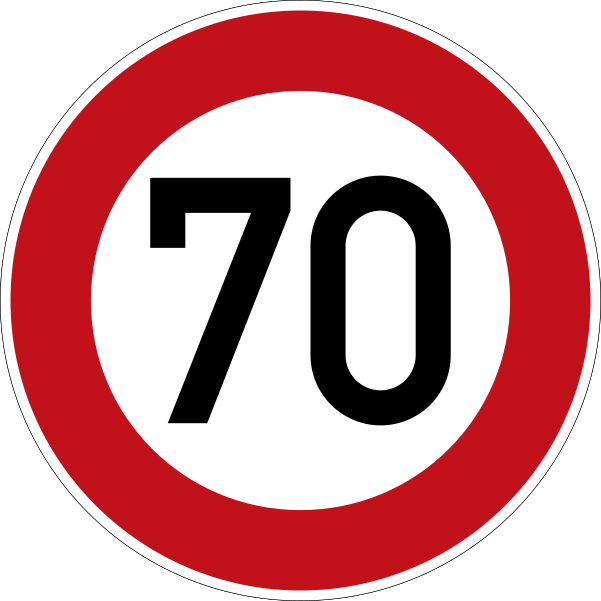
\includegraphics[width=0.7\linewidth]{imgs/7_real}
\end{subfigure}
\caption{Stop-sign (left) which is misclassified as 'Zulässige Höchstgeschwindigkeit (70)': 99.10\%; true class image (right) for comparison}
\label{fig:stopsign}
\end{figure}